\documentclass[tikz,border=8pt]{standalone}
\definecolor{wall}{HTML}{F6E9D2}
\definecolor{wallshade}{HTML}{EAD9BC}
\definecolor{floor}{HTML}{C9955E}
\definecolor{floordark}{HTML}{A9773F}
\definecolor{rug}{HTML}{C86B5A}
\definecolor{rugline}{HTML}{E9A68E}
\definecolor{sofa}{HTML}{6E8F6B}
\definecolor{sofadark}{HTML}{4F6E4C}
\definecolor{cushion}{HTML}{E9C46A}
\definecolor{skin}{HTML}{F5D6B8}
\definecolor{hair}{HTML}{E6E2DA}
\definecolor{dress}{HTML}{8E6BA8}
\definecolor{dressdark}{HTML}{6C4E86}
\definecolor{tv}{HTML}{2F3640}
\definecolor{screen}{HTML}{7EC8E3}
\definecolor{wood}{HTML}{8B5A2B}
\definecolor{curtain}{HTML}{D98C6B}
\definecolor{curtaindark}{HTML}{B9704F}
\definecolor{lamp}{HTML}{FFE9A8}
\definecolor{lampglow}{HTML}{FFF3C4}
\definecolor{night}{HTML}{3C4E7A}
\begin{document}
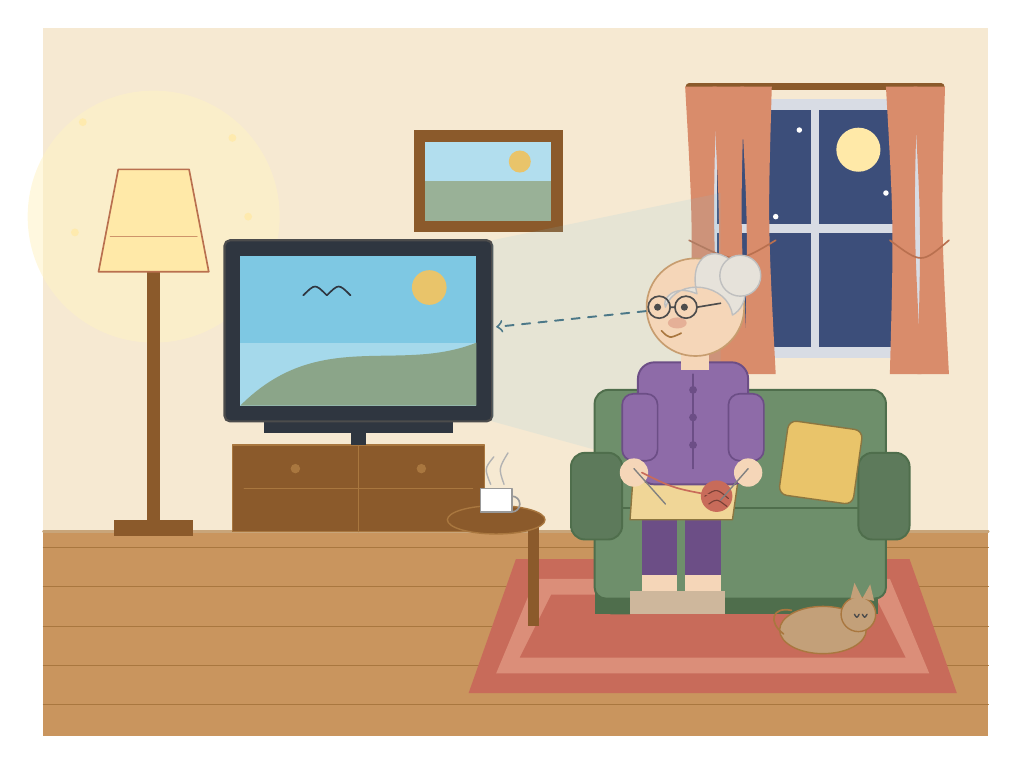
\begin{tikzpicture}[x=1cm,y=1cm,line join=round,line cap=round]
  % room: 12 x 9
  \fill[wall] (0,0) rectangle (12,9);
  \fill[wallshade] (0,0) rectangle (12,0.6);
  \fill[floor] (0,0) rectangle (12,2.6);
  \foreach \y in {0.4,0.9,1.4,1.9,2.4}{\draw[floordark,line width=0.4pt] (0,\y) -- (12,\y);}
  \draw[floordark!60!wall,line width=1pt] (0,2.6) -- (12,2.6);

  % window with curtains (upper right)
  \fill[night] (8.4,4.8) rectangle (11.2,8.1);
  \fill[white!80!night] (8.4,4.8) rectangle (11.2,8.1);
  \fill[night] (8.55,4.95) rectangle (11.05,7.95);
  \fill[lamp] (10.35,7.45) circle (0.28);
  \foreach \p in {(9.0,7.4),(9.6,7.7),(10.7,6.9),(9.3,6.6)}{\fill[white] \p circle (0.035);}
  \draw[white!80!night,line width=3pt] (9.8,4.95) -- (9.8,7.95) (8.55,6.45) -- (11.05,6.45);
  \draw[wood,line width=2.5pt] (8.2,8.25) -- (11.4,8.25);
  \foreach \x in {8.2,8.55,8.9}{\fill[curtain] (\x,4.6) .. controls (\x+0.05,6.5) .. (\x-0.05,8.25) -- (\x+0.35,8.25) .. controls (\x+0.3,6.5) .. (\x+0.4,4.6) -- cycle;}
  \foreach \x in {10.75,11.1}{\fill[curtain] (\x,4.6) .. controls (\x+0.05,6.5) .. (\x-0.05,8.25) -- (\x+0.35,8.25) .. controls (\x+0.3,6.5) .. (\x+0.4,4.6) -- cycle;}
  \draw[curtaindark,line width=0.6pt] (8.2,6.3) .. controls (8.8,6.0) .. (9.3,6.3);
  \draw[curtaindark,line width=0.6pt] (10.75,6.3) .. controls (11.15,6.0) .. (11.5,6.3);

  % wall picture frame
  \fill[wood] (4.7,6.4) rectangle (6.6,7.7);
  \fill[white!85!wall] (4.85,6.55) rectangle (6.45,7.55);
  \fill[sofa!70!white] (4.85,6.55) rectangle (6.45,7.05);
  \fill[screen!60!white] (4.85,7.05) rectangle (6.45,7.55);
  \fill[cushion] (6.05,7.3) circle (0.14);

  % floor lamp (left of TV, warm glow)
  \fill[lampglow,opacity=0.55] (1.4,6.6) circle (1.6);
  \fill[wood] (1.32,2.6) rectangle (1.48,6.0);
  \fill[wood] (0.9,2.55) rectangle (1.9,2.75);
  \fill[lamp,draw=curtaindark,line width=0.6pt] (0.7,5.9) -- (2.1,5.9) -- (1.85,7.2) -- (0.95,7.2) -- cycle;
  \draw[curtaindark!70!lamp,line width=0.5pt] (0.85,6.35) -- (1.95,6.35);

  % TV cabinet + TV (left)
  \fill[wood,draw=floordark,line width=0.6pt] (2.4,2.6) rectangle (5.6,3.7);
  \draw[floordark,line width=0.5pt] (4.0,2.6) -- (4.0,3.7) (2.55,3.15) -- (5.45,3.15);
  \fill[floordark] (3.2,3.4) circle (0.06) (4.8,3.4) circle (0.06);
  \fill[tv] (2.8,3.85) rectangle (5.2,4.05);
  \fill[tv] (3.9,3.7) rectangle (4.1,3.95);
  \fill[tv,draw=black!70,line width=0.8pt,rounded corners=2pt] (2.3,4.0) rectangle (5.7,6.3);
  \fill[screen] (2.5,4.2) rectangle (5.5,6.1);
  % on-screen scene: sunny hill with a bird
  \fill[white!30!screen] (2.5,4.2) rectangle (5.5,5.0);
  \fill[sofa!80!white] (2.5,4.2) .. controls (3.5,5.2) and (4.5,4.6) .. (5.5,5.0) -- (5.5,4.2) -- cycle;
  \fill[cushion] (4.9,5.7) circle (0.22);
  \draw[tv,line width=0.6pt] (3.3,5.6) .. controls (3.45,5.75) .. (3.6,5.6) (3.6,5.6) .. controls (3.75,5.75) .. (3.9,5.6);
  % TV glow onto the room
  \fill[screen,opacity=0.13] (5.7,4.0) -- (8.6,3.2) -- (8.6,6.9) -- (5.7,6.3) -- cycle;

  % rug
  \fill[rug] (5.4,0.55) -- (11.6,0.55) -- (11.0,2.25) -- (6.0,2.25) -- cycle;
  \fill[rugline,opacity=0.6] (5.75,0.8) -- (11.25,0.8) -- (10.75,2.0) -- (6.25,2.0) -- cycle;
  \fill[rug] (6.05,1.0) -- (10.95,1.0) -- (10.55,1.8) -- (6.45,1.8) -- cycle;

  % side table with teacup (between sofa and TV)
  \fill[wood] (6.15,1.4) rectangle (6.3,2.8);
  \fill[wood,draw=floordark,line width=0.5pt] (5.75,2.75) ellipse (0.62 and 0.18);
  \fill[white,draw=black!40,line width=0.5pt] (5.55,2.85) rectangle (5.95,3.15);
  \draw[black!40,line width=0.6pt] (5.95,3.05) arc (90:-90:0.1);
  \draw[black!30,line width=0.5pt] (5.68,3.2) .. controls (5.6,3.4) .. (5.72,3.55);
  \draw[black!30,line width=0.5pt] (5.85,3.2) .. controls (5.78,3.4) .. (5.9,3.6);

  % sofa (right, facing the TV = facing left)
  \fill[sofadark] (7.0,1.55) rectangle (10.6,1.85);
  \fill[sofa,draw=sofadark,line width=0.7pt,rounded corners=4pt] (7.0,1.75) rectangle (10.7,3.05);
  \fill[sofa,draw=sofadark,line width=0.7pt,rounded corners=5pt] (7.0,2.9) rectangle (10.7,4.4);
  \fill[sofa!85!black,draw=sofadark,line width=0.7pt,rounded corners=5pt] (6.7,2.5) rectangle (7.35,3.6);
  \fill[sofa!85!black,draw=sofadark,line width=0.7pt,rounded corners=5pt] (10.35,2.5) rectangle (11.0,3.6);
  \fill[cushion,draw=cushion!60!black,line width=0.5pt,rounded corners=3pt,rotate around={-8:(9.9,3.5)}] (9.4,3.0) rectangle (10.35,3.95);
  \fill[sofadark] (7.2,1.55) rectangle (7.45,1.75) (10.25,1.55) rectangle (10.5,1.75);

  % grandmother sitting on the sofa, body turned toward the TV (left)
  % legs
  \fill[dressdark] (7.6,1.75) rectangle (8.05,2.95);
  \fill[dressdark] (8.15,1.75) rectangle (8.6,2.95);
  \fill[skin] (7.6,1.85) rectangle (8.05,2.05);
  \fill[skin] (8.15,1.85) rectangle (8.6,2.05);
  \fill[hair!60!floordark] (7.45,1.55) rectangle (8.1,1.85);
  \fill[hair!60!floordark] (8.05,1.55) rectangle (8.65,1.85);
  % lap blanket
  \fill[cushion!70!white,draw=cushion!60!black,line width=0.5pt] (7.45,2.75) -- (8.75,2.75) -- (8.85,3.45) -- (7.5,3.45) -- cycle;
  % torso (cardigan)
  \fill[dress,draw=dressdark,line width=0.7pt,rounded corners=6pt] (7.55,3.2) rectangle (8.95,4.75);
  \draw[dressdark,line width=0.5pt] (8.25,3.4) -- (8.25,4.6);
  \fill[dressdark] (8.25,3.7) circle (0.05) (8.25,4.05) circle (0.05) (8.25,4.4) circle (0.05);
  % arms: one resting on lap, other holding a tea cup / knitting
  \fill[dress,draw=dressdark,line width=0.6pt,rounded corners=4pt] (7.35,3.5) rectangle (7.8,4.35);
  \fill[skin] (7.5,3.35) circle (0.18);
  \fill[dress,draw=dressdark,line width=0.6pt,rounded corners=4pt] (8.7,3.5) rectangle (9.15,4.35);
  \fill[skin] (8.95,3.35) circle (0.18);
  % neck + head (in profile-ish 3/4 view, looking left toward TV)
  \fill[skin] (8.1,4.65) rectangle (8.45,4.95);
  \fill[skin,draw=floordark!60!skin,line width=0.6pt] (8.28,5.45) circle (0.62);
  % hair bun (grey)
  \fill[hair,draw=black!25,line width=0.5pt] (8.3,5.62) .. controls (8.15,6.25) and (8.75,6.3) .. (8.9,5.75) .. controls (8.95,5.55) and (8.85,5.4) .. (8.75,5.35) .. controls (8.7,5.75) and (8.05,5.85) .. (7.9,5.45) .. controls (7.85,5.55) and (8.0,5.75) .. (8.3,5.62) -- cycle;
  \fill[hair,draw=black!25,line width=0.5pt] (8.85,5.85) circle (0.26);
  % glasses + eye looking left, gentle smile, cheek
  \draw[black!70,line width=0.6pt] (7.82,5.45) circle (0.14);
  \draw[black!70,line width=0.6pt] (8.16,5.45) circle (0.14);
  \draw[black!70,line width=0.6pt] (7.96,5.45) -- (8.02,5.45) (8.3,5.45) -- (8.6,5.5);
  \fill[black!70] (7.8,5.45) circle (0.045) (8.14,5.45) circle (0.045);
  \draw[floordark,line width=0.6pt] (7.85,5.15) .. controls (7.95,5.05) .. (8.1,5.12);
  \fill[rug,opacity=0.35] (8.05,5.25) ellipse (0.12 and 0.07);
  % gaze line toward the TV
  \draw[screen!60!black,dashed,line width=0.7pt,->] (7.65,5.4) -- (5.75,5.2);

  % knitting in her hands (yarn ball on lap)
  \fill[rug] (8.55,3.05) circle (0.2);
  \draw[rug!60!black,line width=0.4pt] (8.4,3.05) .. controls (8.55,3.15) .. (8.7,3.02) (8.45,2.95) .. controls (8.55,3.02) .. (8.68,2.92);
  \draw[black!50,line width=0.5pt] (7.5,3.4) -- (7.9,2.95) (8.95,3.4) -- (8.6,3.0);
  \draw[rug,line width=0.6pt] (7.6,3.35) .. controls (8.0,3.15) .. (8.55,3.05);

  % cat curled on the rug
  \fill[floordark!70!white,draw=floordark,line width=0.5pt] (9.9,1.35) ellipse (0.55 and 0.3);
  \fill[floordark!70!white,draw=floordark,line width=0.5pt] (10.35,1.55) circle (0.22);
  \fill[floordark!70!white] (10.25,1.75) -- (10.3,1.95) -- (10.4,1.75) -- cycle (10.4,1.75) -- (10.5,1.93) -- (10.55,1.72) -- cycle;
  \draw[floordark,line width=0.6pt] (9.4,1.3) .. controls (9.2,1.45) and (9.25,1.65) .. (9.5,1.6);
  \draw[black!70,line width=0.5pt] (10.3,1.55) .. controls (10.33,1.5) .. (10.36,1.55) (10.4,1.55) .. controls (10.43,1.5) .. (10.46,1.55);

  % a few warm light particles from the lamp
  \foreach \p in {(0.5,7.8),(2.4,7.6),(2.6,6.6),(0.4,6.4)}{\fill[lamp,opacity=0.8] \p circle (0.05);}
\end{tikzpicture}
\end{document}
